
\documentclass [12pt, proquest]{uwthesis}[2019]

\usepackage{graphicx}
\usepackage{subfig}
\usepackage{amsmath}
\usepackage{setspace}
\usepackage{lineno}
\usepackage{natbib}

\begin{document}

\title{}
\prelimpages
 
\Title{Development and Deployment of Precision Mechanical Rotation Sensor for Terrestrial Gravitational Wave Observatories}
\Author{M. P. Ross}
\Year{2019}
\Program{Physics}

\Chair{Name of Chairperson}{Title of Chair}{Department of Chair}
\Signature{First committee member}
\Signature{Next committee member}
\Signature{etc}

\copyrightpage

\titlepage  

\setcounter{page}{-1}
\abstract{}

\tableofcontents
\listoffigures

\dedication{\begin{center}To Grace\end{center}}
\textpages
\chapter{Introduction}
\section{Gravitational Wave Theory}
\section{Seismic Isolation}

\chapter{1-m Scale Ground Rotation Sensors}
\section{Tilt Contamination}
\quad At their core seismometers are low frequency spring mass system which measures the difference in motion between the casing and the device's proof mass. Above the resonant frequency of the spring mass system, this allows for accurate measurements of the motion in reference to an inertial frame of any object that the casing is rigidly connected to, be it the ground or a suspended table. Over the past \textbf{some time} this technology has produced devices that are sensitive to \textbf{number and range}. However, these systems are fundamentally susceptible to any stray forces acting on the proof mass.

Of interest here is the contamination due to the rotation of the device within a external gravitational field, namely the field caused by the earth. The rotation in respect to a fixed gravitational force will be referred to as tilt.\footnote{Although a subtle difference, the distinction would be of great consequences if the local gravitational field was varying rapidly. In that case the sensors described here would be of little use as they are rotational sensors not tilt sensors.} From the proof mass's frame, a tilt is equivalent to a rotation of the gravitational force. This yields a horizontal acceleration of the proof mass of:
\[ a=g \text{ sin}(\theta)\]
where $g$ is the gravitational acceleration on the surface of the earth and $\theta$ is the angle that the device is rotated. This acceleration adds a second term to the seismometer's output shown below for small angles and in the Fourier domain:
\[\tilde{x}_{seis}(\omega)=\tilde{x}_{trans}(\omega)+\frac{g}{\omega^2}\tilde{\theta}_{wind}(\omega)\]
where $x_{seis}$ is the seismometer's output, $x_{trans}$ is the translational motion of the device, and $\omega$ is the frequency at which the tilt is being driven. 

With this additional contribution, it becomes immediately clear that, for a given amplitude of tilt, the contamination term contributes more at lower frequencies and readily dominates the translational signal. In the context of the ground seismometers at the observatory, the tilt signal swamps the translational component below $\sim$ 100 mHz. Above which the seismometer signal is dominate by the ever present oceanic microseism which is driven by low frequency pressure waves with the ocean and their interaction with the shoreline. \textbf{CITE} This can be seen in Figure \ref{wind} which shows an amplitude spectral density of a ground seismometer at LHO during both low and high wind conditions.

\begin{figure}%
\begin{center}
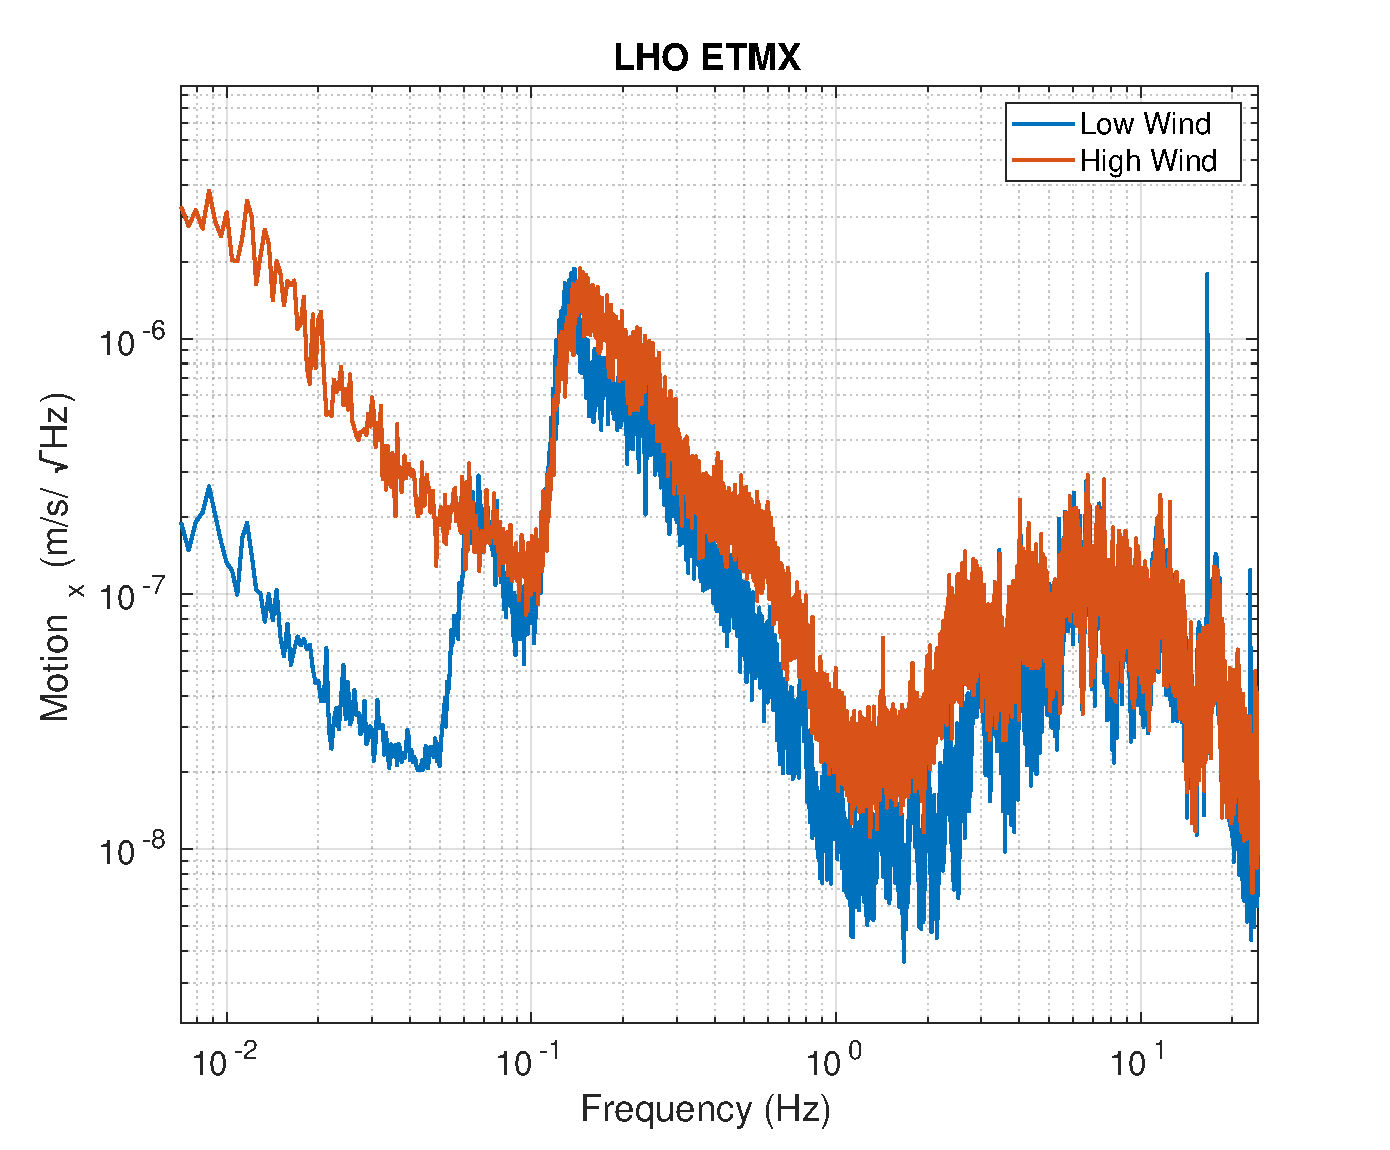
\includegraphics[width=0.5\textwidth]{windComp.pdf}
\caption{}
\label{wind}
\end{center}
\end{figure}

The dominate driver of ground tilts at the observatories is wind acting on the walls of the building. Although one would naiively assume that the wind would rigidly rotate the building, it was found that the true mechanism is differential pressure acting on the walls deforms the building's concrete slab. \textbf{cite?} 

\section{Sensor Correction with Tilt Subtraction}

\quad There are a few different ways to combat such a contamination. The most straight forward is to decrease the wind pressure by designing builds that don't interact with the wind as much or installing wind blocks such as wind fences or earth burms. Both of these option require significant construction and for the case of LIGO, tilt contamination was not known to be a problem when design the observatories. Another option is to build seismometers that are suspended in such a way that they do not experience tilts. This is an active area of research and may yield tilt-free seismometers. \textbf{cite}

The scheme that will be used here is to measure the tilt with an independent rotation sensor and subtract the wind driven contribution. This would then yield a channel of the following form:
\begin{align}
x_{seis}(\omega)=x_{trans}(\omega)+&\frac{g}{\omega^2}\theta_{wind}(\omega)\\
-&\frac{g}{\omega^2}\theta_{meas}(\omega)
\end{align}

where $\theta_{meas}$ is the tilt seen by the rotation sensor. Given a coherence $\gamma$ between the tilt component of the seismometer and rotation sensors this yields the following: \textbf{CHECK math}

\[x_{seis}(\omega)=x_{trans}(\omega)+\frac{g}{\omega^2}(1-\gamma)\theta_{wind}(\omega)\]

This is then a low tilt channel which can be used within the LIGO seismic isolation system.

\section{Mechanical System}

The Beam Rotation Sensor (BRS) is a beam balance comprised of a 1-m long beam hung from two 10-15 $\mu$m thick beryllium-copper flexures. Figure \textbf{number} shows a CAD model of the beam balance. 

\textbf{BRS image}

This design makes the beam stiff in all degrees of freedom other than rotations around the horizontal axis which intersects the two flexure pivot points. This forms a system consisting of two elementary subsystems: a rotational spring mass system formed by the stiffness of the flexures, and a simple pendulum due to the offset of the pivot point and the center of mass. This is then described by the following equation of motion: \cite{venk2014}

\[I \ddot{\theta}(t)+\kappa (1+ \frac{i}{Q})(\theta(t)-\theta_p(t))+M g \delta \theta(t) +M \delta \ddot{x_p}(t)=\tau_{ex}(t)\]

where $\theta$ and $\theta_p$ are, respectively, the angle of beam and the platform with respect to gravitational vertical, $\tau_{ext}$ is the sum of all exterior torques, $I$ is the moment of inertia, $Q$ is the quality factor of the system, $\kappa$ is the spring constant of the flexures, $M$ is the mass of the balance, $g$ is the gravitational acceleration, $\delta$ is the vertical distance from the center of mass and the pivot point, and $x_p$ is the translation of the platform.

\textbf{derive translational coupling and readout equation}

In ideal operation, one would tune the center of mass to be at the pivot point and thus would produce a pure rotational spring-mass system with no translational coupling. In this limit, the rotation sensor is a rotational analog to a seismometer; above the resonant frequency as the casing rotates the beam stays inertial and thus allows one to measure the casing's rotation.

\section{Multi-Slit Autocollimator Readout}

\quad Optical levers are a simple optical angular readout which exploits the law of reflection to measure angular deflections of a mirror by observing the displacement of a reflected beam. The angle of the mirror is then described as:
\[\theta_{mirror}=\frac{x_{reflected}}{2d}\]
where $\theta_{mirror}$ is the angle of the mirror, $x_{reflected}$ is the displacement of the reflected beam, and $d$ is the distance between the optical system and the mirror. This allows one to increase the precious of the angular measurements arbitrarily by increasing $d$. However, with this comes a few disadvantages. One the effective gain of the sensor depends of the $d$ which may not be well known. Additionally, the system is sensitive to changes in $d$. 

An autocollimator adds a lens located one focal length from light source and the screen, shown in Figure \textbf{number}. This effectively replace the distance dependence with the focal length of the lens which allows the system to be only sensitive, to first order, to the angular motion of the mirror.

\textbf{autocollimator schematic}

To improve upon this further, a partially reflective mirror can be placed in between the optical system and the main mirror to act as a reference and allows for the subtraction of any motion of the optical system with respect to the main mirror. This yield a angular readout described by:
\[\theta_{mirror}=\frac{x_{main}-x_{reference}}{2f}\]

where $f$ is the focal length of the lens and $x_{reference}$ is the beam spot from the reference mirror.

An increase in sensitivity can be made by employing a multi-slit autocollimator \textbf{cite MSA paper}. This consists of an autocollimator with the light source replaced by a illuminated photomask of a number of thin slits. The pattern is then reflected off a set of reference and main mirror and imaged by a line CCD camera. These images are then analyzed to measure the distance between them thus yielding a measurement of angle. For the BRSs, this image analysis is achieved using bespoke software written in C\# which can be found at www.github.com/mpross/BRSReadout

To extract the distance between the patterns, the image goes through a series of steps to go from a vector of pixel intensities to a single angular output. When the software begins, the first frame that is captured is saved to compare all future frames to. 

\textbf{make table of BRS autocollimator parameters: focus, number of slits, slit width, CCD type, light source}

\section{Controls}
\section{Noise Performance}
\section{Hanford Installation}
\section{Livingston Installation}

\chapter{30-cm Scale On-Board Rotation Sensors}
\section{Angular Controls}
\section{Mechanical System}
\section{Interferometric Readout}
\section{Controls}
\section{Noise Performance}

\chapter{Applications}
\section{Geophysics}
\subsection{Rayleigh Wave Theory}
\subsubsection{Wave Field Parameter Extraction}
\subsection{Single Station Dispersion Measurements}
\section{Newtonian Noise}
\subsection{Theory}
\subsection{Observations}

\bibliographystyle{apalike}
\bibliography{Dissertation}
\printendnotes
\nocite{*}   
\bibliographystyle{plain}
\bibliography{Dissertation}
\end{document}


